\section*{TL;DR if you're new}

This is minesweeper\\
\begin{figure}[h]
    \centering
    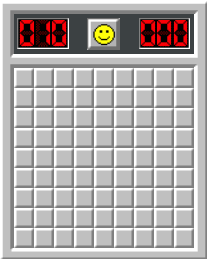
\includegraphics{figures/1/empty_board.PNG}
\end{figure}

This is a mine. They occupy some spaces of the board.\\
\begin{figure}[h]
    \centering
    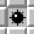
\includegraphics{figures/1/mine.PNG}
\end{figure}

Play by clicking squares. Numbers say how many of the neighboring squares (including diagonals) have mines.\\
\begin{figure}[h]
    \centering
    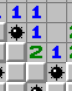
\includegraphics{figures/1/example.PNG}
\end{figure}

Win by uncovering all squares without mines.\\


\vspace{10em}
{\huge DO NOT READ ANY FURTHER}\\

I strongly encourage you to play and learn the game yourself. IMO this is the best way to have fun playing minesweeper.

